PLC is used to control the subsystems in the robotic workcell. PLC controls the bending process by controlling the bending machine,
operates the unloading station to get new sheet metal parts to the unloading station gripper using the gantry robot, triggers the inspection camera for testing the bending process and cooperates with the KR1410 to select the correct bending task. To achieve all of this, communication needs to be setup between various subsystems. Figure \ref{fig:communication-protocols} shows the networking diagram between various devices in the workcell. ROS PC has not been commissioned in the robotic workcell, but a setup could easily be made by connecting an ethernet cable between
robot controller and laptop.


\begin{figure}[h]
  \centering
  \begin{tikzpicture}[
      device/.style={draw, rectangle, minimum width=2.5cm, minimum height=1cm, align=center},
      connection/.style={thick}, % bidirectional arrows
      protocol/.style={above, sloped, font=\small\ttfamily},
      ip/.style={font=\small} % IP address style
    ]
    
    % Devices without IP inside node
    \node[device] (PLC) {PLC};
    \node[device, below=2cm of PLC] (KR1410) {KR1410};
    \node[device, right=3cm of PLC] (InspectionCamera) {Inspection Camera};
    \node[device, below=2cm of KR1410] (RoboticCamera) {Robotic Camera};
    \node[device, below=2cm of InspectionCamera] (PC) {ROS PC};
    
    % Web UI node
    \node[device, below=2cm of PC] (WebUI) {Web UI};
    
    % IP addresses outside nodes
    \node[ip, above=0.0cm of PLC] {192.168.0.102};
    \node[ip, above left=-0.55cm and 0cm of KR1410] {192.168.0.120};
    \node[ip, below left=-0.55cm and 0.0cm of KR1410] {192.168.39.1};
    \node[ip, above=0.0cm of InspectionCamera] {192.168.0.101};
    \node[ip, below=0.0cm of RoboticCamera] {192.168.0.100};
    \node[ip, right=0.0cm of PC] {192.168.39.42};
    \node[ip, below=0.0cm of WebUI] {http://localhost:3000};

    % Connections
    \draw[connection] (PLC) -- (KR1410) node[protocol, midway] {Profinet};
    \draw[connection] (KR1410) -- (RoboticCamera) node[protocol, midway] {Ethernet};
    \draw[connection] (KR1410) -- (PC) node[protocol, midway] {Ethernet};
    \draw[connection] (PLC) -- (InspectionCamera) node[protocol, midway] {Profinet};
    \draw[connection] (PC) -- (WebUI) node[protocol, midway] {Websocket};
    
    \end{tikzpicture}
  \caption{System Networking and IP Addressing}
  \label{fig:communication-protocols}
\end{figure}


\begin{table}[h]
  \centering
  \small
  \renewcommand{\arraystretch}{1.2} % Adjusts row height
  \begin{tabular}{l@{\hskip 2cm}l}
    \hline
      \textbf{Input Register} & \textbf{Function} \\ \hline
      \multicolumn{2}{c}{\textbf{Bit}} \\ \hline
      Bit[0] & open or close unloading station gripper \\
      Bit[1] & open or close robotic gripper\\
      Bit[2] & bending start request/release\\
      Bit[3] & inspection camera trigger request/release\\
      Bit[4] & robot active\\
      Bit[5] & sheet request\\\hline
      \multicolumn{2}{c}{\textbf{Integer}} \\ \hline
      \textbf{Int[0]} & \textbf{Current robot state in program}\\
      Int[0]=0 & Not ready or failure\\
      Int[0]=1 & getting to ready pose\\
      Int[0]=2 & waiting for new sheet\\
      Int[0]=3 & performing bending operation 1\\
      Int[0]=4 & performing bending operation 2\\
      Int[0]=5 & performing bending operation 3\\
      Int[0]=6 & performing bending operation 4\\
      Int[0]=7 & performing bending operation 5\\
      Int[0]=8 & performing bending operation 6\\
      Int[0]=9 & placing sheet metal part in shelf\\
      Int[0]=10 & performing calibration\\
      \textbf{Int[1]} & \textbf{Robotic camera trigger state}\\
      Int[1]=0 & no trigger\\
      Int[1]=1 & successful, object detected\\
      Int[1]=2 & failure, object not detected\\
      \textbf{Int[2]} & \textbf{Robotic camera operation state}\\
      Int[2]=0 & Working\\
      Int[2] is not 0 & Not working, camera restart required\\
      \hline
  \end{tabular}
  \caption{Sending data from KR1410 to PLC over Profinet}
  \label{tab:kr1410-to-plc}
\end{table}

\begin{table}[h!]
  \centering
  \small
  \renewcommand{\arraystretch}{1.2} % Adjusts row height
  \begin{tabular}{c@{\hskip 2cm}l}
    \hline
      \textbf{Output Register} & \textbf{Function} \\ \hline
      \multicolumn{2}{c}{\textbf{Bit}} \\ \hline
      % Bit[0]-Bit-[7] & Cutoff for bending machine open height \\
      % &  value from laser sensor for each \\
      % & bending operation\\
      % & 1 - above cutoff, bending station engaged,\\
      % & regrasp sheet after bending\\
      % & 0 - below cutoff, hold sheet in backgauge \\
      \textbf{Bit[0]-Bit-[7]} & \textbf{trigger for bending machine reaching a}\\
      & \textbf{certain open height value determined}\\
      & \textbf{using laser sensor} \\
      Bit[0] & Bending operation 1 started\\
      Bit[1] & Bending operation 2 started\\
      Bit[2] & Bending operation 3 started\\
      Bit[3] & Bending operation 4 started\\
      Bit[4] & Bending operation 5 started\\
      Bit[5] & Bending operation 6 started\\
      Bit[6] & Bending finished, take out sheet\\
      Bit[7] & Bending machine fully open\\
      Bit[8] & Start bending sequence program\\
      Bit[9] & Sheet metal ready in unloading\\
      & station gripper\\
      Bit[10] & Correcting bending machine sequence\\
      & using terminal robot\\
      Bit[11] & Inspecting requested\\
      Bit[12] & Pause program\\
      Bit[13] & Calibration requested\\
      Bit[14] & Terminate program\\
      Bit[15] & Storage station secured\\
      \hline
      \multicolumn{2}{c}{\textbf{Integer}} \\ \hline
      \textbf{Int[0]} & \textbf{Inspection Results}\\
      Int[0]=0 & Waiting for results\\
      Int[0]=1 & Successful\\
      Int[0]=2 & Failure\\
      \hline
  \end{tabular}
  \caption{Sending data from PLC to KR1410 over Profinet}
  \label{tab:plc-to-kr1410}
\end{table}

\subsection{Communication between KR1410 Robot and PLC}
The communication between the PLC and KR1410 is established over Profinet, a leading industrial ethernet protocol for communication between devices in industrial automation systems. Profinet (usually styled as PROFINET, as a portmanteau for Process Field Net) ensures real-time data transmission and supports various network topologies. \cite{profinet}

A number of robot data can be monitored and controller through PLC over Profinet. These include monitoring of system state, joint configuration,
TCP kinematics, IO Board, Tool IO state, and controlling of master speed, IO Board, and Tool IO outputs. The profinet also allows the transfer of
data from Robot to PLC over user defined 64 Bit Input, 24 Int Input, 24 Real Input and from PLC to Robot over 64 Bit Output, 24 Int Output and 24 Real Output. \cite{kr-profinet} Table \ref{tab:kr1410-to-plc} and \ref{tab:plc-to-kr1410} shows the defined variables for cooperation between PLC and KR1410 which are shared over profinet.


\subsection{VISOR Communication Protocols}
Both VISOR camera has been configured beforehand for camera settings like shutter speed, gain, working distance, resolution, internal illumination and other parameters. VISOR has been connected to a PC running SensoConfig software from SENSOPART for configuring the camera.
Using this software, separate jobs could also be added for each task. The task could include detecting a particular sheet pattern, target marker detection or bend angle measurement. CBun \textbf{VISOR} device added to KR teach pendant only allows switching of jobs, triggering camera,
performing calibration and a few other tasks. But training to recognise a pattern needs to be done beforehand using a PC.

\subsubsection{VISOR to KR1410}
Kassow robot is interfaced to the robotic camera using ethernet.
CBun Device installed on KR teach pendant allows for communication between
Kassow robot and the VISOR. It is build and installed using CBun development as mentioned in subsection \ref{subsec:computer-vision}. The following ports are used for communications between the Kassow Robot and the VISOR. 

\begin{itemize}
  \item \textbf{Port 2005}, Transmission control protocol TCP (Implicit results, \textit{i.e.} user-configured result data)
  \item \textbf{Port 2006}, Transmission control protocol TCP (Explicit results, \textit{e.g.} trigger or job switch)
\end{itemize}


\begin{figure}[h]
  \centering
  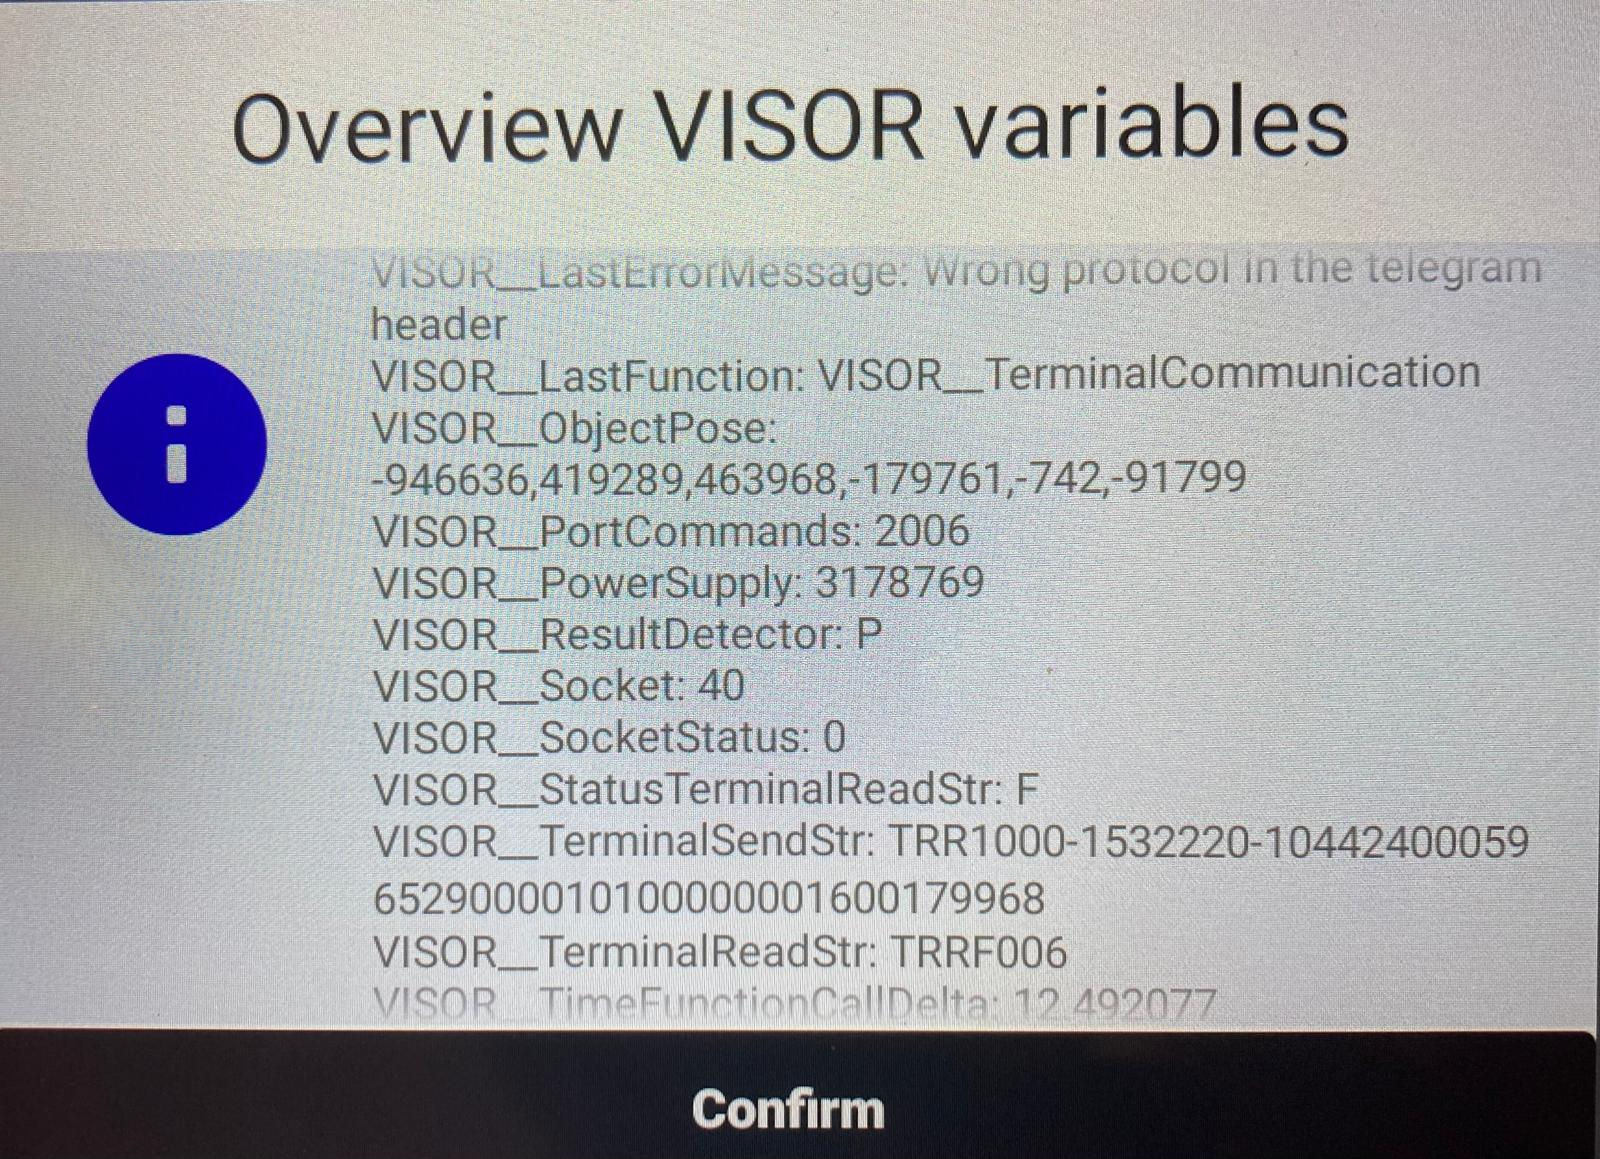
\includegraphics[width=0.55\textwidth]{figures/visor-cbun-connection.png}
  \caption{Dialog Box in teach pendant GUI showing transmission of data over port 2006}
  \label{fig:cbun-variables}
\end{figure}

Figure \ref{fig:calib-graph} shows the use of this communication setup to perform auto-calibration with the Kassow robots and the mounted camera.

\subsubsection{VISOR to PLC}
PLC is interfaced with the inspection camera using Profinet.
UDP (User Datagram Protocol) is used over ports 161, 34962, 34963, 34964 to establish communication between the PLC and the VISOR. \cite{visor_communication_manual}


\subsection{Communication between KR1410 Robot, ROS and Web UI}
\label{subsec:KR1410ROS}

The communication between the Web UI and the nodejs server happens via HTTP for standard page loading. The websocket connection through rosbridge provides real-time, bidirectional data exchange between the real or simulated robot and the web interface. This allows visualization, monitoring
and also control of the robot through web application. Figure \ref{fig:ros-web-graph} shows the communication diagram between ROS, Web application and the KR.

\begin{figure}[h]
  \centering
  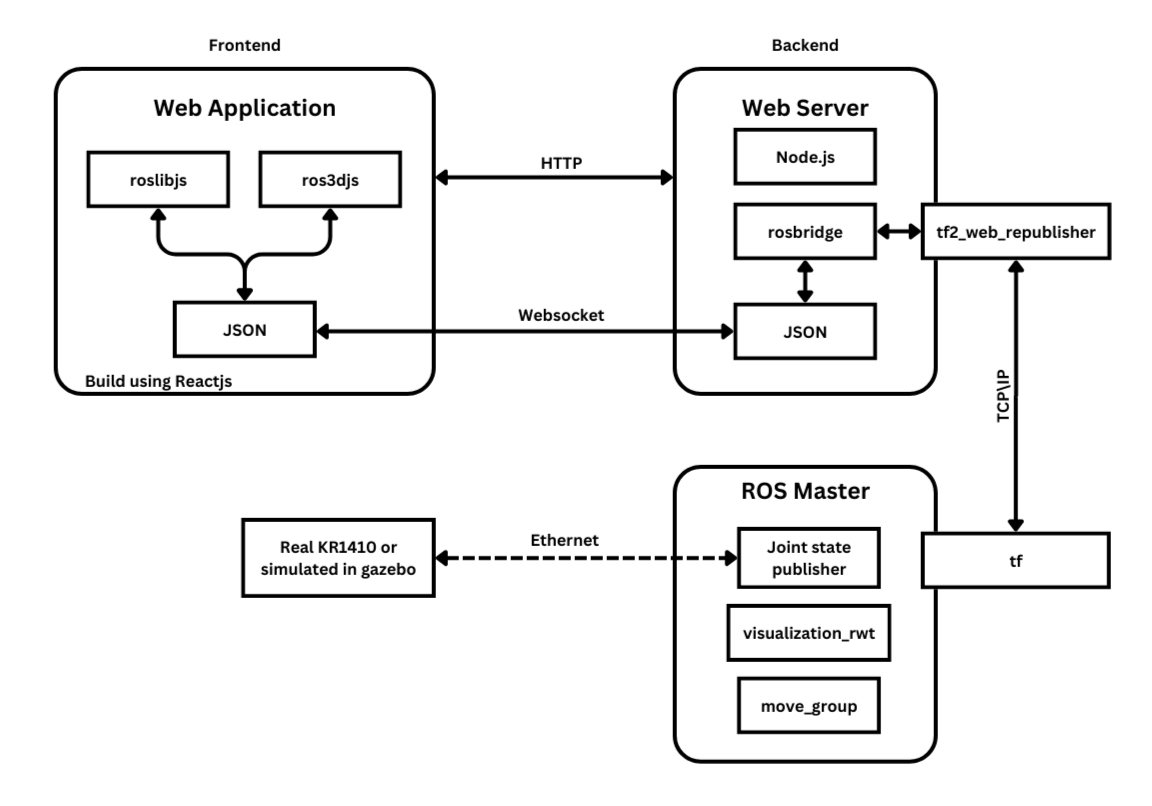
\includegraphics[width=1\textwidth]{figures/ros-web-graph.png}
  \caption{ROS connection to KR1410 and web UI}
  \label{fig:ros-web-graph}
\end{figure}

Web UI is build using the frontend development tool ReactJS. It utilizes libraries like \hyperref[par:roslibjs]{\textbf{roslibjs}} and \hyperref[par:ros3djs]{\textbf{ros3djs}} to visualize or publish on ROS topics which monitors or controls the robot respectively. Rosbridge acts as a bridge between the web application and the ROS system. It converts ROS messages into JSON format which can be sent over the websocket.

ROS nodes uses either TCP/IP or UDP communication protocol. 
The ROS Master acts as the central node manager in the ROS network. It coordinates communication between the robot (KR1410) and other ROS nodes.
Here the machine running ROS provides the ROS master \cite{rosmaster} and the KR1410 robot is connected to it through ethernet where KR ROS support provides few nodes and rostopics through which real robot can be monitored and controlled. These topics are republished to \textit{joint\_state\_publisher} so that they can be controlled using MoveIt package.
KR1410 could also be simulated in gazebo software for testing of the web UI. Gazebo also publishes joints on \textit{joint\_states\_publisher} which are used in ROS and MoveIt to control the robot.

A number of ROS nodes runs on the ROS machine which includes MoveIt nodes, unloading station gripper controller nodes, \textit{visualization\_rwt} for MoveIt controls through the Web UI, \textit{joint\_state\_controller}, \textit{robot\_state\_controller}, rosbridge, \textit{tf2\_web\_publisher} etc. Nodes are written in python or C++. \textit{robot\_state\_controller} publishes the state of the robot on \textbf{tf} rostopic using \textit{joint\_states} and parameter \textit{robot\_description}. The \textbf{tf} (transform) rostopic is responsible for managing transforms between different links of the robot. \textit{tf2\_web\_publisher} uses this rostopic to recreate the robot in the web application.

